\section{Nachhaltigkeit}

Das wiederverwenden von Material trägt Massgeblich dazu bei Abfall zu reduzieren. Bei der Konstruktion der Grundplatte wurde darauf


\begin{figure}[H] % oder [htbp]
    \centering
    \begin{subfigure}[b]{0.45\textwidth}
        \centering
        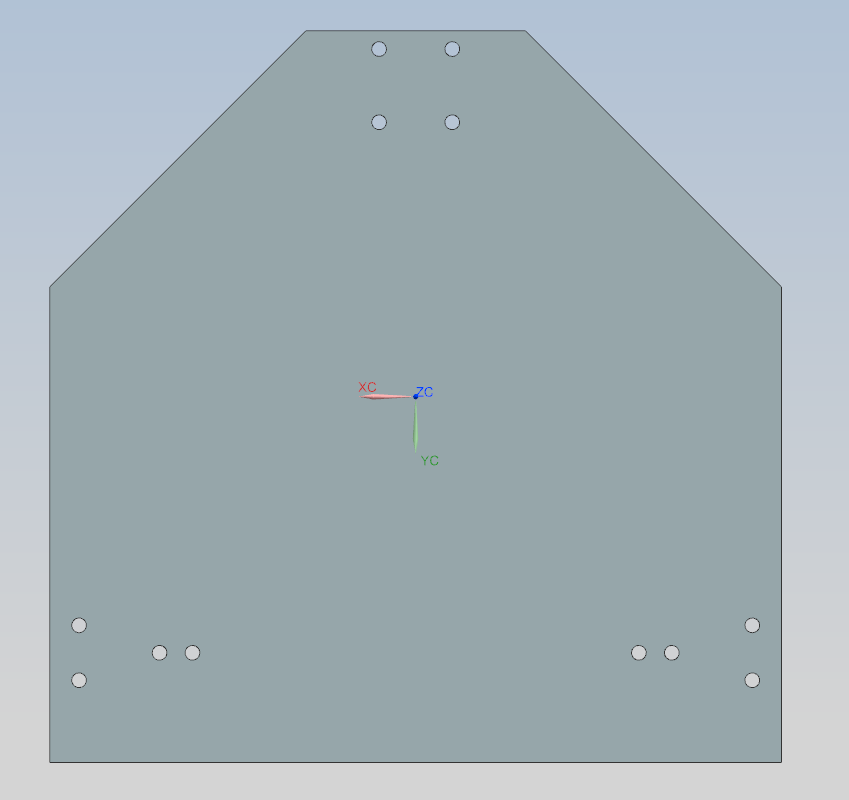
\includegraphics[width=\linewidth]{Grundplatte_V0}
        \caption{Grundplatte V0}
    \end{subfigure}
    \hfill
    \begin{subfigure}[b]{0.45\textwidth}
        \centering
        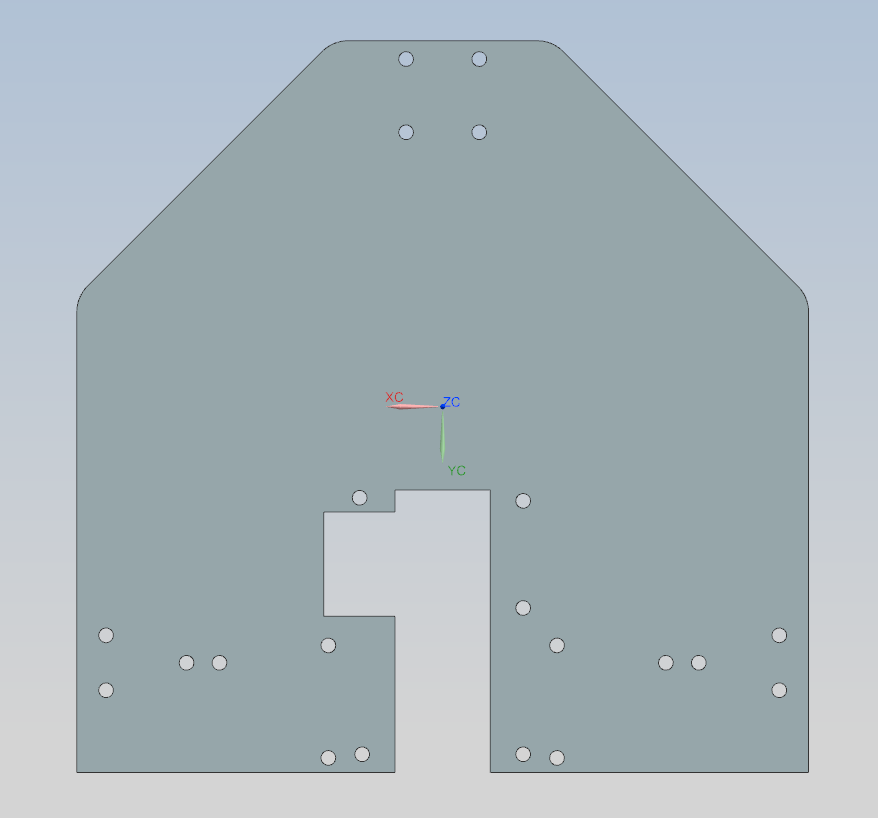
\includegraphics[width=\linewidth]{assets/MT/Grundplatte_V1.png}
        \caption{Grundplatte V1}
    \end{subfigure}

    \vspace{0.5cm}

    \begin{subfigure}[b]{0.45\textwidth}
        \centering
        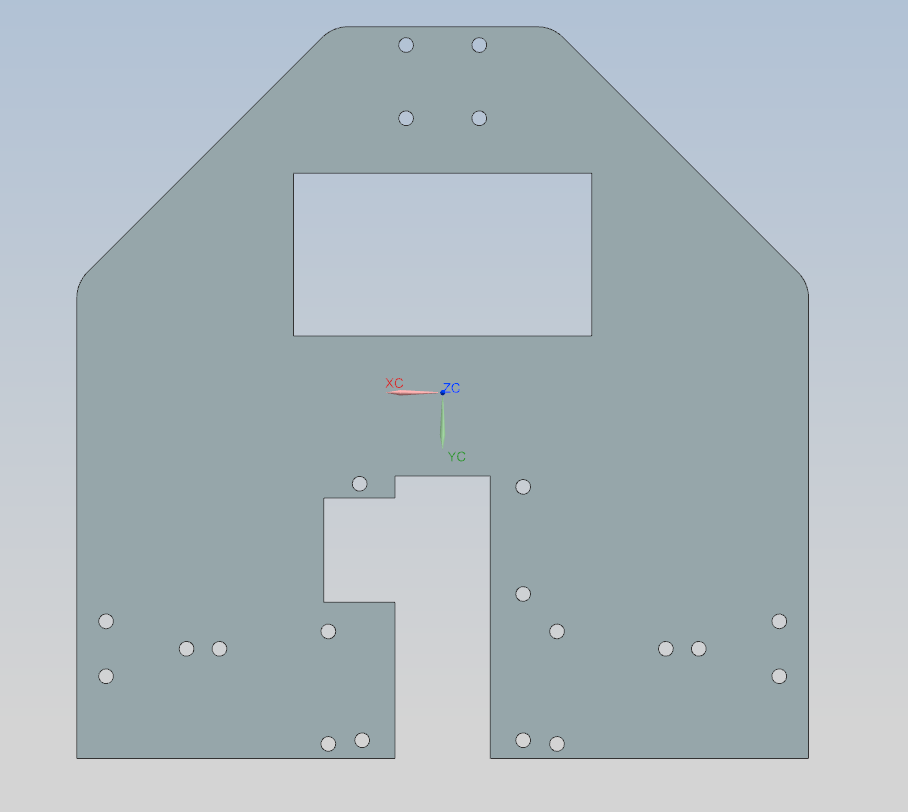
\includegraphics[width=\linewidth]{assets/MT/Grundplatte_V2.png}
        \caption{Grundplatte V2}
    \end{subfigure}
    \hfill
    \begin{subfigure}[b]{0.45\textwidth}
        \centering
        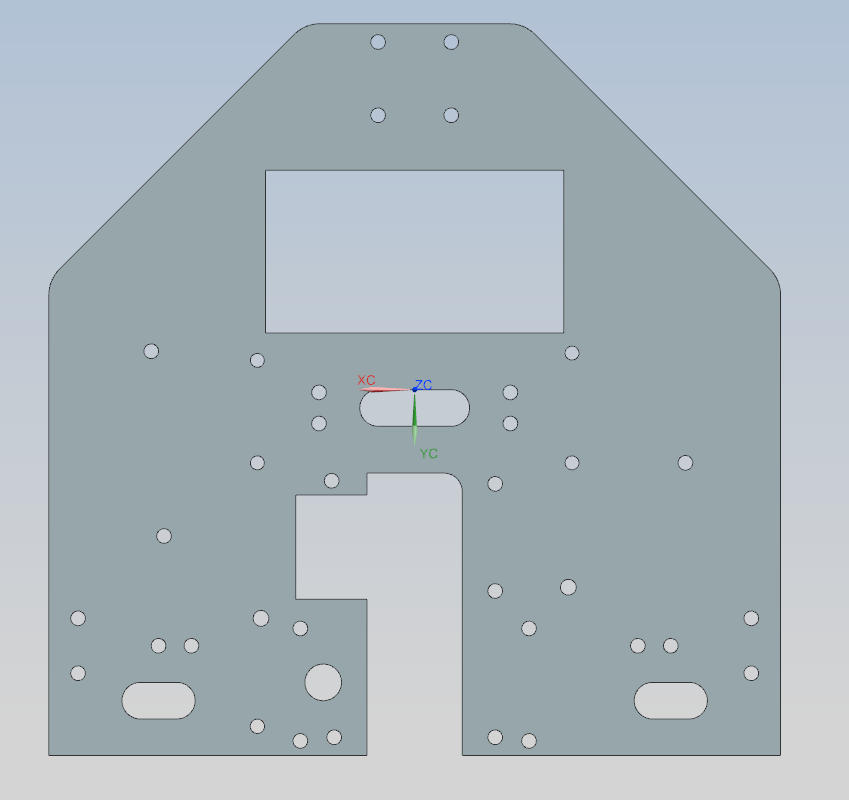
\includegraphics[width=\linewidth]{assets/MT/Grundplatte_V3.png}
        \caption{Grundplatte V3}
    \end{subfigure}
    \caption{Vier Bilder im Quadrat}
\end{figure}

\subsection{Oekobilanz}

Was gibt es alles und wie viel davon?

Was ist recyclebar? ...

3 Mengemaessig meiste (gewicht?)

3 schlechteste

min 2 Seiten